\documentclass[12pt,a4paper]{report}

% -------------------------------------------------
% Packages
% -------------------------------------------------
\usepackage[a4paper,margin=1in]{geometry}
\usepackage{graphicx}
\usepackage{hyperref}
\usepackage{amsmath,amssymb}
\usepackage{listings}
\usepackage{xcolor}
\usepackage{enumitem}
\usepackage{setspace}
\usepackage{titlesec}
\usepackage{float}

% -------------------------------------------------
% Code block style
% -------------------------------------------------
\lstdefinelanguage{Python}{
  morekeywords={import,from,def,return,for,while,if,else,elif,in,not,and,or,
    with,as,class,True,False,None,lambda,try,except,raise},
  keywordstyle=\color{blue}\bfseries,
  comment=[l]{\#},
  stringstyle=\color{orange}\ttfamily,
  commentstyle=\color{gray}\ttfamily,
}

\lstdefinelanguage{SQL}{
  morekeywords={SELECT,FROM,WHERE,JOIN,ON,AND,OR,GROUP,BY,HAVING,SUM,AS},
  keywordstyle=\color{blue}\bfseries,
  morestring=[b]',
  stringstyle=\color{orange}\ttfamily,
}

\lstdefinelanguage{Bash}{
  morekeywords={python3},
  keywordstyle=\color{blue}\bfseries,
  comment=[l]{\#},
  stringstyle=\color{orange}\ttfamily,
}

\lstset{
  language=Python,
  basicstyle=\ttfamily\small,
  frame=single,
  breaklines=true,
  numbers=left,
  numberstyle=\tiny\color{gray},
  keywordstyle=\color{blue}\bfseries,
  stringstyle=\color{orange},
  commentstyle=\color{gray}\itshape,
  tabsize=2,
  showstringspaces=false
}

\hypersetup{
  colorlinks=true,
  linkcolor=blue,
  urlcolor=blue
}

% -------------------------------------------------
% Title Page Information
% -------------------------------------------------
\title{
\textbf{CSIT6910}\\[6pt]
\Large Independent Project Report\\[6pt]
\textbf{R2T-Based Differentially Private Query Evaluation on TPC-H}
}
\author{
Name: \underline{Xu Dongliu}\\
Student ID: \underline{21208710}\\[6pt]
Instructor: \underline{Ke Yi}\\
Semester: \underline{2025-26 Spring}
}
\date{\today}

\begin{document}

\maketitle
\tableofcontents
\newpage

% =============================================================
\chapter{Project Overview}

\section{Project Title}
\textit{R2T-Based Differentially Private Query Evaluation on TPC-H}

\section{Background}

Differential privacy protects the contribution of one private entity when
query answers are released. In relational databases with foreign-key
constraints, one entity may be connected to many secondary tuples. For
example, one customer may reference many orders, and each order may
reference many lineitems. Removing this customer therefore changes a
join-and-aggregate query by more than one tuple.

The R2T (Race-to-the-Top) algorithm addresses this issue by adaptively
choosing a truncation threshold. For each candidate threshold $\tau$, the
query answer is truncated so that one private entity can contribute at
most $\tau$. R2T then adds calibrated Laplace noise and a penalty term,
and returns the best noisy candidate. This project applies the R2T idea
to two TPC-H revenue queries.

\section{Project Scope}

The implementation focuses on two concrete TPC-H cases rather than a
general SQL engine. Both cases designate \texttt{Customer} as the private
relation. The queries are adapted from TPC-H Query 3 and Query 5: the
TPC-H join structure and predicates are preserved, while the final output
is converted to a scalar revenue aggregate suitable for R2T release.

\begin{figure}[H]
  \centering
  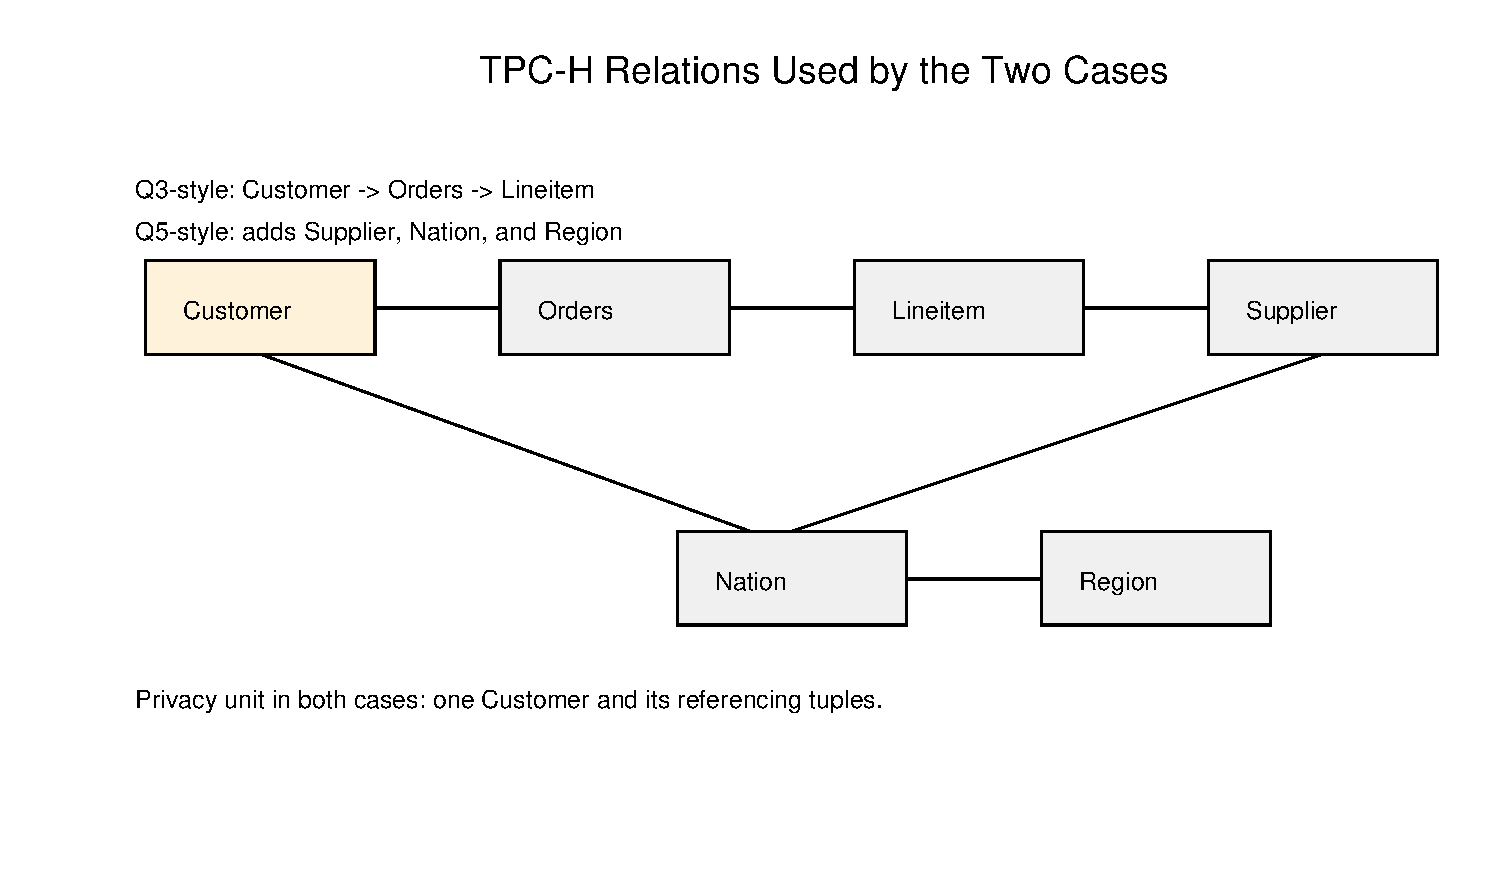
\includegraphics[width=0.9\textwidth]{figures/schema_cases.pdf}
  \caption{Relations used in the two implemented TPC-H cases}
\end{figure}

% =============================================================
\chapter{Algorithm Design}

\section{Algorithm Overview}

\begin{figure}[H]
  \centering
  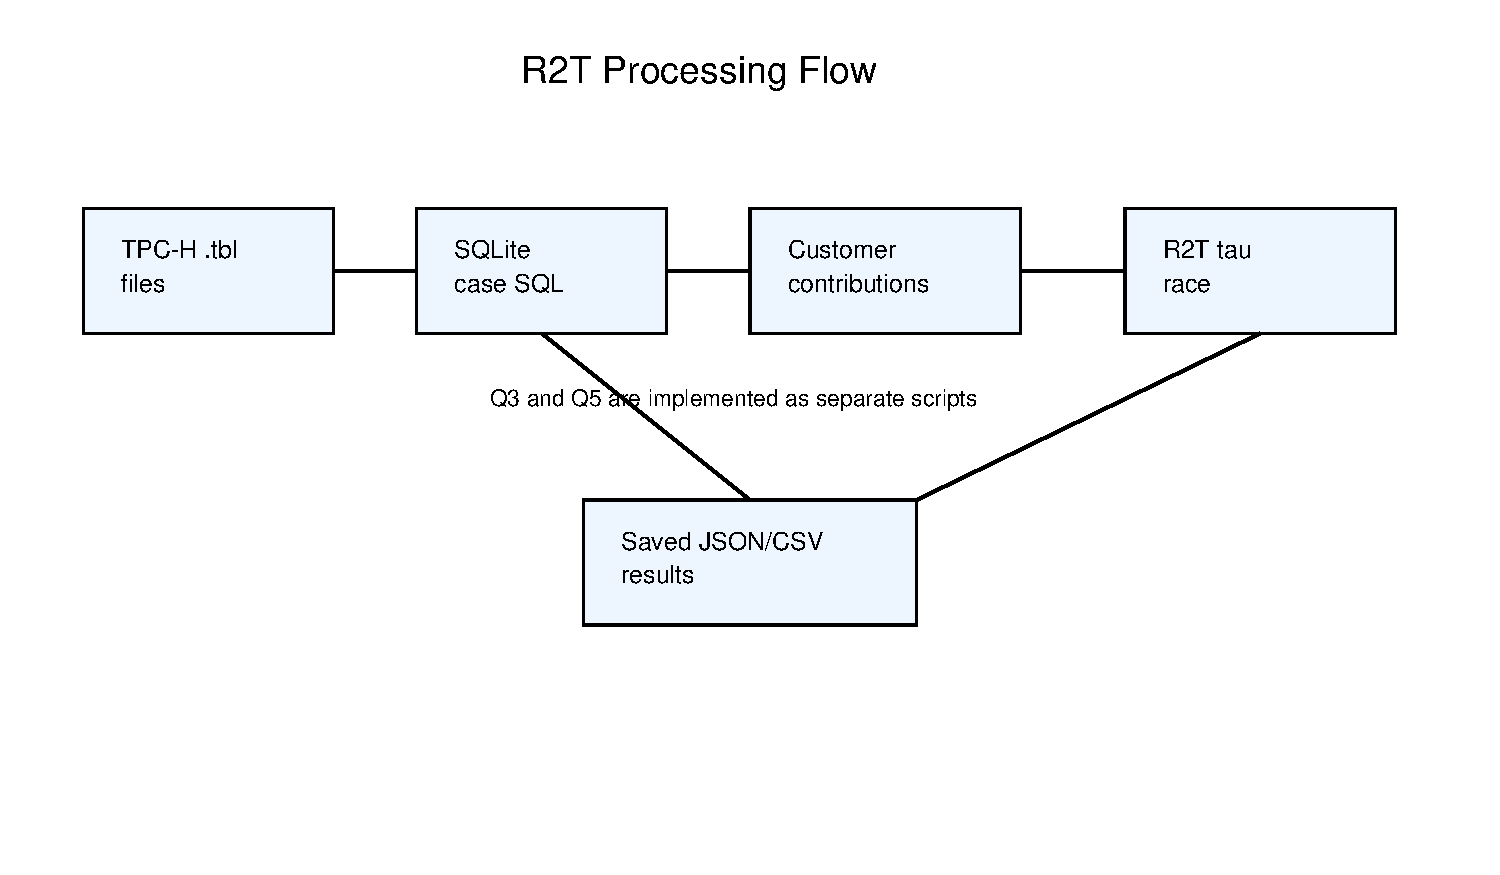
\includegraphics[width=0.9\textwidth]{figures/algorithm_flow.pdf}
  \caption{Implementation flow of the R2T-based query evaluation}
\end{figure}

For each case, the program first loads the required TPC-H \texttt{.tbl}
files into an in-memory SQLite database. It then executes a case-specific
SQL query to compute each customer's contribution to the revenue. Let
$x_i$ be the revenue contribution of customer $i$. For a candidate
threshold $\tau$, the truncated answer is
\[
Q(I,\tau) = \sum_i \min(x_i,\tau).
\]
Because the implemented cases are self-join-free and protect customers,
this closed-form truncation is equivalent to the corresponding linear
programming solution for these cases.

R2T evaluates candidates $\tau = 2,4,8,\ldots,2^{\lfloor
\log_2(GS_Q)\rfloor}$. For each $\tau$, it computes
\[
\widetilde{Q}(I,\tau)
= Q(I,\tau)
+ Lap\left(\frac{\log_2(GS_Q)\tau}{\epsilon}\right)
- \log_2(GS_Q)\ln\left(\frac{\log_2(GS_Q)}{\beta}\right)
\frac{\tau}{\epsilon}.
\]
The final output is
\[
\max \left(0, \max_\tau \widetilde{Q}(I,\tau)\right),
\]
where $Q(I,0)=0$ for the positive revenue queries used here.

\section{Implemented Cases}

\subsection{TPC-H Q3-Style Customer Revenue}

This case uses \texttt{Customer}, \texttt{Orders}, and \texttt{Lineitem}.
It keeps customers in the \texttt{BUILDING} market segment, orders before
1995-03-15, and lineitems shipped after 1995-03-15.

\begin{lstlisting}[language=SQL]
SELECT c.C_CUSTKEY,
       SUM(l.L_EXTENDEDPRICE * (1.0 - l.L_DISCOUNT)) AS revenue
FROM Customer c
JOIN Orders o ON c.C_CUSTKEY = o.O_CUSTKEY
JOIN Lineitem l ON o.O_ORDERKEY = l.L_ORDERKEY
WHERE c.C_MKTSEGMENT = 'BUILDING'
  AND o.O_ORDERDATE < '1995-03-15'
  AND l.L_SHIPDATE > '1995-03-15'
GROUP BY c.C_CUSTKEY;
\end{lstlisting}

\subsection{TPC-H Q5-Style ASIA Revenue}

This case uses \texttt{Customer}, \texttt{Orders}, \texttt{Lineitem},
\texttt{Supplier}, \texttt{Nation}, and \texttt{Region}. It keeps ASIA
region records from 1994 and requires the customer and supplier to belong
to the same nation.

\begin{lstlisting}[language=SQL]
SELECT c.C_CUSTKEY,
       SUM(l.L_EXTENDEDPRICE * (1.0 - l.L_DISCOUNT)) AS revenue
FROM Customer c
JOIN Orders o ON c.C_CUSTKEY = o.O_CUSTKEY
JOIN Lineitem l ON o.O_ORDERKEY = l.L_ORDERKEY
JOIN Supplier s ON l.L_SUPPKEY = s.S_SUPPKEY
JOIN Nation n ON c.C_NATIONKEY = n.N_NATIONKEY
             AND s.S_NATIONKEY = n.N_NATIONKEY
JOIN Region r ON n.N_REGIONKEY = r.R_REGIONKEY
WHERE r.R_NAME = 'ASIA'
  AND o.O_ORDERDATE >= '1994-01-01'
  AND o.O_ORDERDATE < '1995-01-01'
GROUP BY c.C_CUSTKEY;
\end{lstlisting}

% =============================================================
\chapter{Experiment Design and Outcome}

\section{Experiment Setup}

The implementation is written in Python and uses only the standard
library: \texttt{sqlite3}, \texttt{csv}, \texttt{json}, \texttt{math}, and
\texttt{random}. The input data comes from the local TPC-H tables under
\texttt{BDT\_IP\_Differential-privacy/data}. The default parameters are
$\epsilon=0.8$, $\beta=0.1$, $GS_Q=10{,}000{,}000$, and random seed 1.

The main commands are:

\begin{lstlisting}[language=Bash]
python3 code/case_q3_customer_revenue.py --seed 1
python3 code/case_q5_asia_revenue.py --seed 1
python3 code/validate_cases.py
\end{lstlisting}

Each case writes a JSON summary and a CSV file of all R2T candidates to
the \texttt{results/} directory.

\section{Validation Design}

The validation script checks implementation-level invariants for both
cases. It verifies that each query has positive output, that truncated
answers never exceed the original SQL total, that truncated answers are
monotone as $\tau$ increases, and that the per-customer truncation bound
$Q(I,\tau) \leq \tau \cdot |\{customers\}|$ holds. These checks passed
for both implemented cases.

\section{Experimental Results}

\begin{table}[H]
\centering
\begin{tabular}{|l|r|r|}
\hline
\textbf{Metric} & \textbf{Q3-style} & \textbf{Q5-style} \\ \hline
Contributing customers & 904 & 655 \\ \hline
True SQL total & 114,904,912.53 & 30,276,617.68 \\ \hline
Maximum customer contribution & 661,967.22 & 210,018.26 \\ \hline
Selected $\tau$ & 131,072 & 65,536 \\ \hline
Truncated value at selected $\tau$ & 81,707,181.04 & 26,148,964.08 \\ \hline
R2T noisy output & 63,926,157.02 & 14,653,924.70 \\ \hline
\end{tabular}
\caption{Full-data experimental results with seed 1}
\end{table}

\begin{figure}[H]
  \centering
  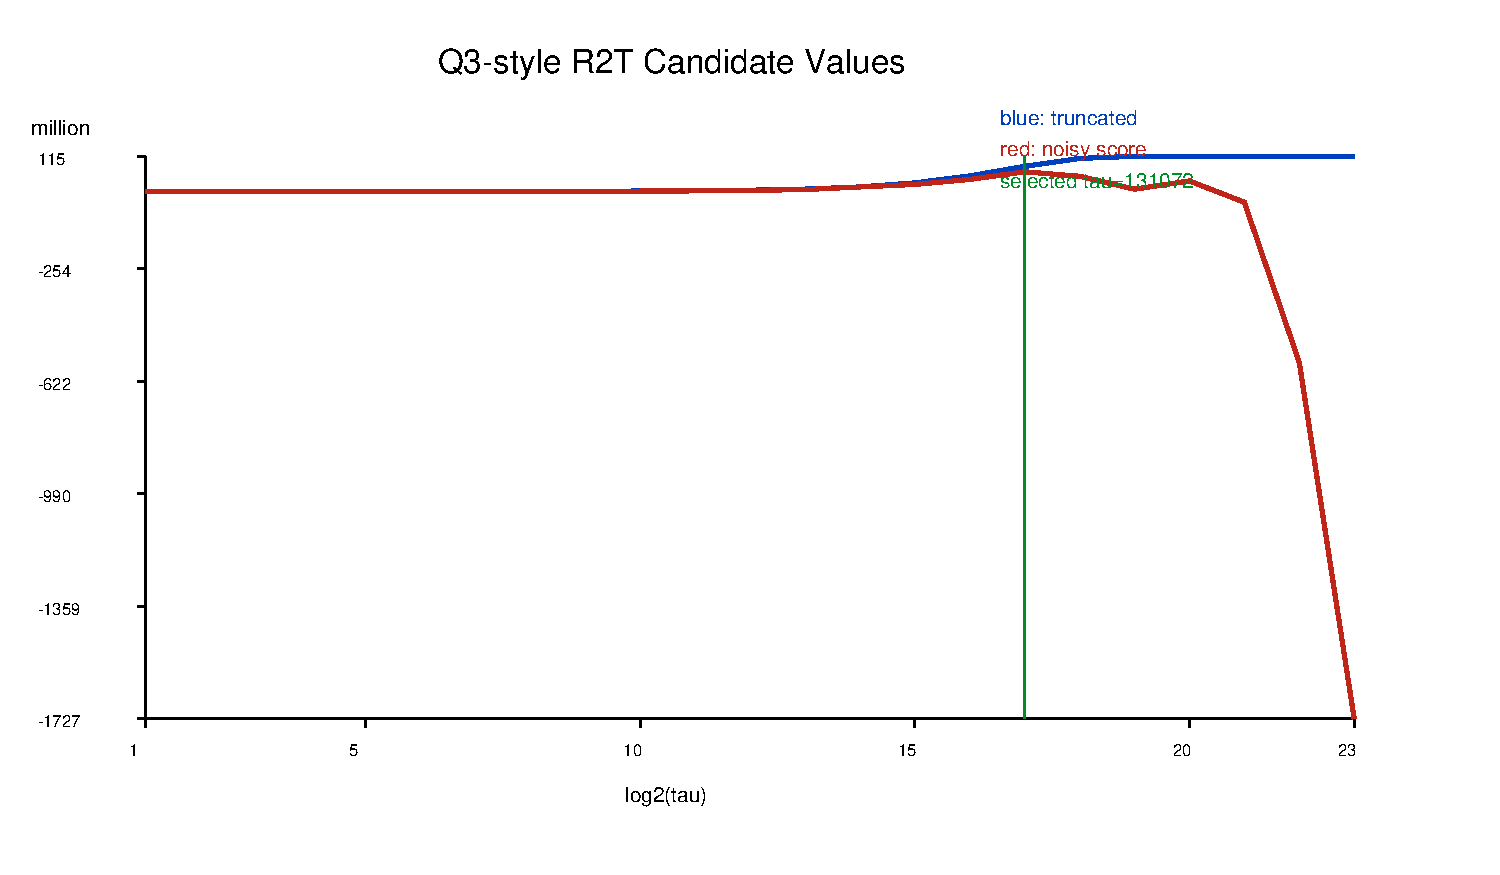
\includegraphics[width=0.9\textwidth]{figures/q3_r2t_candidates.pdf}
  \caption{R2T candidate values for the Q3-style case}
\end{figure}

\begin{figure}[H]
  \centering
  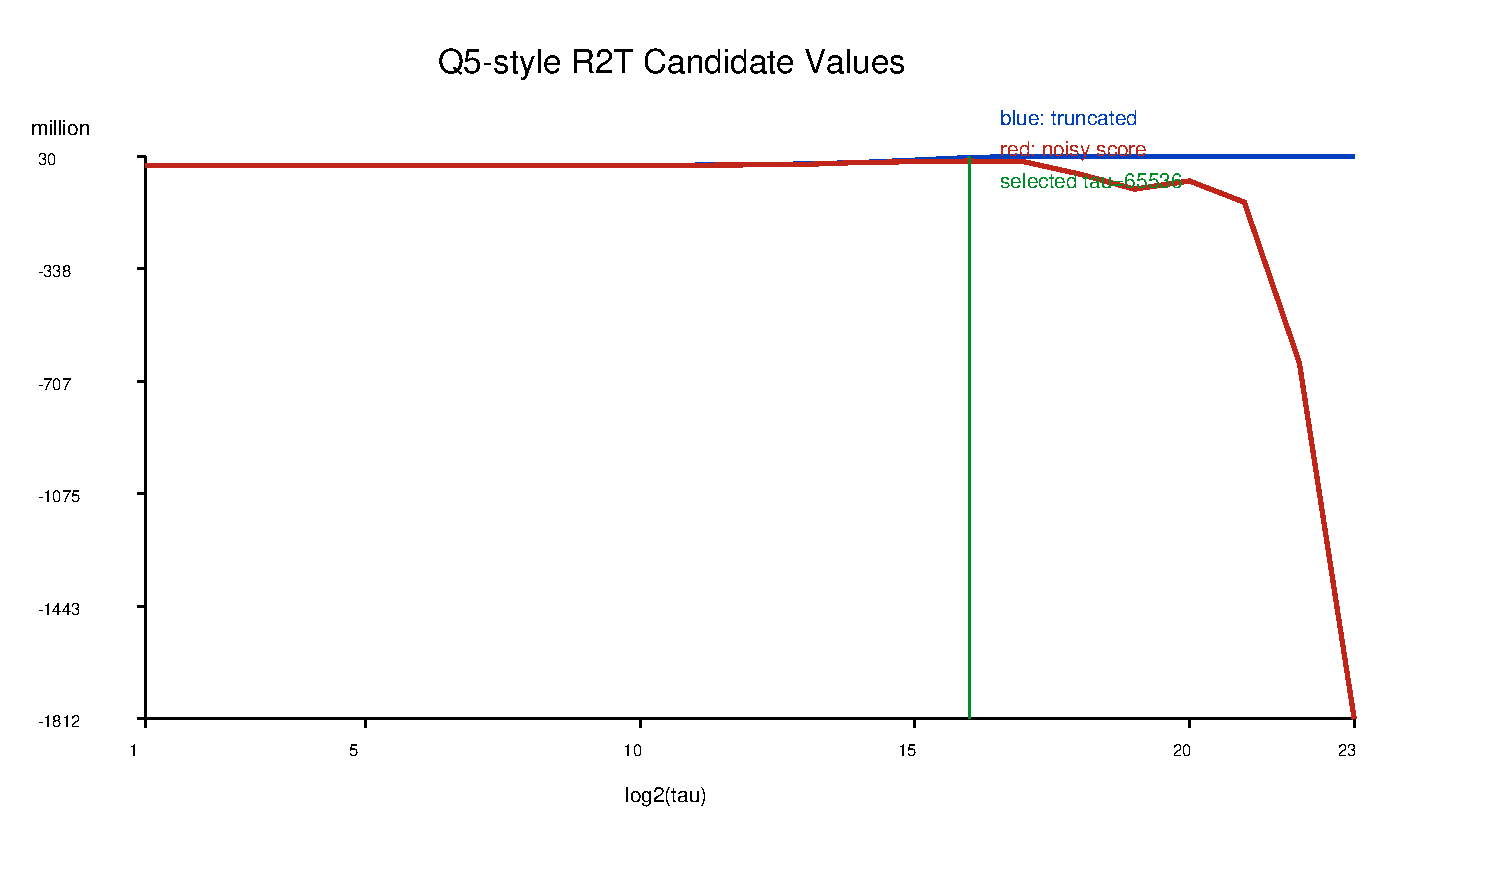
\includegraphics[width=0.9\textwidth]{figures/q5_r2t_candidates.pdf}
  \caption{R2T candidate values for the Q5-style case}
\end{figure}

The selected thresholds are smaller than the point where the truncated
answer fully reaches the original SQL total. This is expected: a larger
$\tau$ reduces truncation bias but increases the Laplace noise scale and
the R2T penalty. The selected threshold is therefore a balance between
accuracy loss from truncation and uncertainty from privacy noise.

\section{Comparison with the Reference Project}

The reference notebook in \texttt{BDT\_IP\_Differential-privacy} was used
only as an implementation reference. It loads TPC-H data with
\texttt{pandas}, runs one Supplier-Lineitem-Orders-Customer revenue join,
solves a linear program using PuLP, and plots R2T-related figures.

This project differs in four ways. First, it implements two separate
TPC-H cases instead of one notebook demo. Second, it uses plain Python
scripts and SQLite rather than a notebook workflow. Third, it does not
copy the reference code or require \texttt{pandas}, \texttt{numpy}, or
\texttt{pulp}. Fourth, for the selected self-join-free customer-private
queries, it uses the equivalent closed-form truncation
$\sum_i \min(x_i,\tau)$ instead of explicitly constructing an LP.

% =============================================================
\chapter{Conclusion}

This project implemented R2T-style differentially private query
evaluation for two TPC-H revenue queries. The implementation loads local
TPC-H data, computes customer-level contributions, performs the R2T
threshold race, saves reproducible JSON and CSV outputs, and validates
key truncation invariants. The result demonstrates how R2T can be applied
to concrete foreign-key relational queries without building a full SQL
privacy engine.

% =============================================================
\appendix
\chapter{Meeting Minutes}

\section{Minutes of the 1st Project Meeting}
\begin{center}
\textbf{Meeting Minutes}
\end{center}

\begin{tabular}{ll}
\textbf{Date}: & Saturday, February 7, 2026 \\
\textbf{Time}: & 4:00 pm \\
\textbf{Place}: & Zoom meeting \\
\textbf{Present}: & Xu Dongliu \\
\textbf{Apology}: & None \\
\textbf{Note-taker}: & Xu Dongliu \\
\end{tabular}

\section*{1. Approval of Minutes}
This was the first project meeting, so there were no previous minutes to approve.

\section*{2. Discussion Items}
\subsection*{Project Direction}
The meeting discussed the project topic, the R2T paper, and the plan to use TPC-H data for differential privacy experiments. The initial task was to understand the algorithm and inspect the available reference implementation.

\section*{3. Meeting Adjournment and Next Meeting}
The meeting adjourned at 4:45 pm. The next meeting was planned for March.

\newpage

\section{Minutes of the 2nd Project Meeting}
\begin{center}
\textbf{Meeting Minutes}
\end{center}

\begin{tabular}{ll}
\textbf{Date}: & Tuesday, March 17, 2026 \\
\textbf{Time}: & 3:00 pm \\
\textbf{Place}: & Zoom meeting \\
\textbf{Present}: & Xu Dongliu \\
\textbf{Apology}: & None \\
\textbf{Note-taker}: & Xu Dongliu \\
\end{tabular}

\section*{1. Approval of Minutes}
The minutes of the first meeting were reviewed. No changes were needed.

\section*{2. Discussion Items}
\subsection*{Algorithm and Data Preparation}
The meeting reviewed the R2T truncation mechanism, the TPC-H schema, and the foreign-key relationship from Customer to Orders and Lineitem. The plan was refined to implement two concrete TPC-H cases instead of a general query engine.

\section*{3. Meeting Adjournment and Next Meeting}
The meeting adjourned at 3:45 pm. The next meeting was planned for April.

\newpage

\section{Minutes of the 3rd Project Meeting}
\begin{center}
\textbf{Meeting Minutes}
\end{center}

\begin{tabular}{ll}
\textbf{Date}: & Tuesday, April 21, 2026 \\
\textbf{Time}: & 4:30 pm \\
\textbf{Place}: & Zoom meeting \\
\textbf{Present}: & Xu Dongliu \\
\textbf{Apology}: & None \\
\textbf{Note-taker}: & Xu Dongliu \\
\end{tabular}

\section*{1. Approval of Minutes}
The minutes of the second meeting were reviewed. No changes were needed.

\section*{2. Discussion Items}
\subsection*{Implementation Progress}
The meeting discussed the implementation of the Q3-style and Q5-style TPC-H revenue cases. The main work was to load TPC-H tables, compute customer-level contributions, apply R2T candidate thresholds, and save reproducible result files.

\section*{3. Meeting Adjournment and Next Meeting}
The meeting adjourned at 5:00 pm. The next meeting was planned for May.

\newpage

\section{Minutes of the 4th Project Meeting}
\begin{center}
\textbf{Meeting Minutes}
\end{center}

\begin{tabular}{ll}
\textbf{Date}: & Tuesday, May 19, 2026 \\
\textbf{Time}: & 3:00 pm \\
\textbf{Place}: & Zoom meeting \\
\textbf{Present}: & Xu Dongliu \\
\textbf{Apology}: & None \\
\textbf{Note-taker}: & Xu Dongliu \\
\end{tabular}

\section*{1. Approval of Minutes}
The minutes of the third meeting were reviewed. No changes were needed.

\section*{2. Discussion Items}
\subsection*{Final Report and Results}
The meeting reviewed the final implementation, validation script, generated figures, and saved JSON/CSV outputs. The final report was prepared with experiment results and the public GitHub repository link.

\section*{3. Meeting Adjournment and Next Meeting}
The meeting adjourned at 5:00 pm. This was the final project meeting.

\newpage

\chapter{Project Code and Reproducibility}

\section{Code Layout}

\begin{itemize}
  \item \texttt{code/common.py}: shared data loading, R2T calculation, and result saving.
  \item \texttt{code/case\_q3\_customer\_revenue.py}: Q3-style implementation.
  \item \texttt{code/case\_q5\_asia\_revenue.py}: Q5-style implementation.
  \item \texttt{code/validate\_cases.py}: validation checks.
  \item \texttt{code/generate\_report\_figures.py}: report figure generation.
  \item \texttt{results/}: generated JSON and CSV result files.
  \item \texttt{figures/}: generated PDF figures used in this report.
\end{itemize}

\section{Project Code}

The project code is stored in the local repository directory used for
this report. The main implementation files are under \texttt{code/}, and
the generated outputs are under \texttt{results/}.

Public GitHub repository:
\url{https://github.com/xdl2003/r2t-tpch-dp}

\end{document}
